%% Copernicus Publications Manuscript Preparation Template for LaTeX Submissions
%% ---------------------------------
%% This template should be used for copernicus.cls
%% The class file and some style files are bundled in the Copernicus Latex Package, which can be downloaded from the different journal webpages.
%% For further assistance please contact Copernicus Publications at: production@copernicus.org
%% https://publications.copernicus.org/for_authors/manuscript_preparation.html

%% copernicus_rticles_template (flag for rticles template detection - do not remove!)

%% Please use the following documentclass and journal abbreviations for discussion papers and final revised papers.

%% 2-column papers and discussion papers
\documentclass[, manuscript]{copernicus}



%% Journal abbreviations (please use the same for preprints and final revised papers)


% Advances in Geosciences (adgeo)
% Advances in Radio Science (ars)
% Advances in Science and Research (asr)
% Advances in Statistical Climatology, Meteorology and Oceanography (ascmo)
% Annales Geophysicae (angeo)
% Archives Animal Breeding (aab)
% ASTRA Proceedings (ap)
% Atmospheric Chemistry and Physics (acp)
% Atmospheric Measurement Techniques (amt)
% Biogeosciences (bg)
% Climate of the Past (cp)
% DEUQUA Special Publications (deuquasp)
% Drinking Water Engineering and Science (dwes)
% Earth Surface Dynamics (esurf)
% Earth System Dynamics (esd)
% Earth System Science Data (essd)
% E&G Quaternary Science Journal (egqsj)
% European Journal of Mineralogy (ejm)
% Fossil Record (fr)
% Geochronology (gchron)
% Geographica Helvetica (gh)
% Geoscience Communication (gc)
% Geoscientific Instrumentation, Methods and Data Systems (gi)
% Geoscientific Model Development (gmd)
% History of Geo- and Space Sciences (hgss)
% Hydrology and Earth System Sciences (hess)
% Journal of Bone and Joint Infection (jbji)
% Journal of Micropalaeontology (jm)
% Journal of Sensors and Sensor Systems (jsss)
% Magnetic Resonance (mr)
% Mechanical Sciences (ms)
% Natural Hazards and Earth System Sciences (nhess)
% Nonlinear Processes in Geophysics (npg)
% Ocean Science (os)
% Polarforschung - Journal of the German Society for Polar Research (polf)
% Primate Biology (pb)
% Proceedings of the International Association of Hydrological Sciences (piahs)
% Scientific Drilling (sd)
% SOIL (soil)
% Solid Earth (se)
% The Cryosphere (tc)
% Weather and Climate Dynamics (wcd)
% Web Ecology (we)
% Wind Energy Science (wes)

%% Please DO NOT add additional packages or LaTeX commands to the template. They
%% are not supported by Coperncius. LaTeX packages already
%% included in the copernicus.cls are:
%\usepackage[german, english]{babel}
%\usepackage{tabularx}
%\usepackage{cancel}
%\usepackage{multirow}
%\usepackage{supertabular}
%\usepackage{algorithmic}
%\usepackage{algorithm}
%\usepackage{amsthm}
%\usepackage{float}
%\usepackage{subfig}
%\usepackage{rotating}

% Pandoc citation processing

% The "Technical instructions for LaTex" by Copernicus require _not_ to insert any additional packages.
%%\usepackage{booktabs}
\usepackage{longtable}
\usepackage{array}
\usepackage{multirow}
\usepackage{wrapfig}
\usepackage{float}
\usepackage{colortbl}
\usepackage{pdflscape}
\usepackage{tabu}
\usepackage{threeparttable}
\usepackage{threeparttablex}
\usepackage[normalem]{ulem}
\usepackage{makecell}
\usepackage{xcolor}
%

\begin{document}

\title{Informing IPCC accounting of forest carbon using the global
forest carbon database (ForC v4.0)}


\Author[1]{Madison}{Williams}
\Author[1]{Valentine}{Herrmann}
\Author[1,2]{Rebecca}{Banbury Morgan}
\Author[3]{Ben}{Bond-Lamberty}
\Author[4]{Susan}{Cook-Patton}
\Author[5]{Helene}{Muller-Landau}
\Author[6]{Camille}{Piponiot}
\Author[1]{Teagan}{Rogers}
\Author[1,5 *]{Kristina J.}{Anderson-Teixeira}


\affil[1]{Center for Conservatiton Ecology, Smithsonian Conservation
Biology Institute, Front Royal, VA, United States}
\affil[2]{School of Geography, University of Leeds, Leeds, UK}
\affil[3]{Joint Global Change Research Institute, Pacific Northwest
National Laboratory, College Park, MD, United States}
\affil[4]{The Nature Conservancy; Arlington VA 22203, USA}
\affil[5]{Forest Global Earth Observatory, Smithsonian Tropical Research
Institute, Panama, Republic of Panama}
\affil[6]{CIRAD, Montpellier, France}

\runningtitle{IPCC forest C accounting with ForC}

\runningauthor{Williams et al.}


\correspondence{Kristina J.\ Anderson-Teixeira\ (teixeirak@si.edu)}



\received{}
\pubdiscuss{} %% only important for two-stage journals
\revised{}
\accepted{}
\published{}

%% These dates will be inserted by Copernicus Publications during the typesetting process.


\firstpage{1}

\maketitle


\begin{abstract}
Forests are critical for climate change mitigation and consitute a
substantial portion of planned emissions reductions under the 2015 Paris
Agreement. Yet, the efficacy of greenhouse gas mitigation planning and
reporting is dependent upon the quality of available emission factors
data, including forest carbon (C) stocks and changes therein. Tens of
thousands of relevant forest C estimates have been published, yet are
not readily accesible to the practitioners compiling national greenhouse
gas inventories. Many of these data have, however, been compiled in the
Global Forest C database (ForC; https://forc-db.github.io/) and stand to
be of value to greenhouse gas accounting if made available through the
Emission Factor Database (EFDB) of the International Panel on Climate
Change (IPCC). Here, we develop and document a process for
semi-automated transfer of data from ForC into the EFDB, assess the data
available and transferred to date, and provide recommendations for
improving forest data collection, analysis, and reporting to improve
accounting of forest-sector greenhoouse gas emissions and removals. We
begin by reconciling terminology and mapping ForC fields into EFDB. This
process required some updates to the ForC database structure, leading to
the release of a new version of ForC (v4.0; described here). At the time
of writing, ForC contained \#\# values that would qualify for inclusion
in the EFDB, \#\# of which have been transferred to date. (Some analysis
of representation/ gaps.) In the future, forest C estimates in EFDB can
be improved through targetted research to fill critical gaps, reporting
of information required by IPCC, and continued submission of data from
scientific publications to the EFDB.
\end{abstract}




\introduction[Introduction]

Forests are critical to management of atmospheric concentrations of the
greenhouse gas carbon dioxide (CO\textsubscript{2}), and thereby climate
change. In recent decades, CO\textsubscript{2} uptake by forests,
woodlands, and savannas has exceeded releases from deforestation and
other severe disturbances, resulting in a net carbon CO\textsubscript{2}
sink of \textasciitilde0.88 Gt C yr\textsuperscript{-1} \citep[all
biomes with trees,][]{xu_changes_2021} to \textasciitilde1.6 Gt C
yr\textsuperscript{-1} \citep[forests only,][]{harris_global_2021}. This
has offset an estimated 10\% to 18\% of anthropogenic
CO\textsubscript{2} emissions from fossil fuels and cement
\citep{xu_changes_2021, harris_global_2021}, dramatically slowing the
pace of atmospheric CO\textsubscript{2} accumulation and climate change.
Going into the future, the fate of this important CO\textsubscript{2}
sink is highly uncertain, depending both upon forest responses to
climate change, which are likely to reduce the sink strength
\citep{mcdowell_pervasive_2020, hammond_global_2022}, and on human
conservation, restoration, and management of forests
\citep{ipcc_climate_2019, ipcc_climate_2022}.

Reflecting their strong influence on Earth's climate, forests play a
central role in international plans for climate change mitigation under
the Paris Agreement \citep{unfccc_adoption_2015}. Forest conservation,
reforestation, and improved sustainable management all have significant
-- and relatively cost-effective -- potential as climate change
mitigation options, with conservation and reforestation having the
fourth and fifth largest net emission reduction potentials or all
mitigation options \citep{ipcc_summary_2022}. As of 2016, forest-based
mitigation accounted for 26\% of total planned greenhouse gas mitigation
within Nationally Determined Contributions under the Paris Agreement
\citep{grassi_key_2017}. Yet, envisioned forest-based climate change
mitigation initiatives do not always correspond to actual emission
reductions through on-the-ground implementation
\citep[e.g.,][]{badgley_systematic_2022}. One critical need for ensuring
that forest-based climate change mitigation initiatives are effective is
realistic planning and reporting, underlain by solid scientific data
\citep{anderson-teixeira_effective_2022, deng_comparing_2021}.

The International Panel on Climate Change (IPCC) provides guidance for
national greenhouse gas inventories for reporting to the United Nations
Framework Convention on Climate Change
\citep[UNFCCC,][]{ipcc_2006_2006, ipcc_2019_2019}. Under this guidance,
greenhouse gas inventories include all managed land, including most of
the world's forest land \citep{ogle_delineating_2018}. The IPCC
inventory guidelines include specific instructions for accounting for
greenhouse gas (mainly CO\textsubscript{2}) exchanges between forest
land and the atmosphere \citep{ipcc_agriculture_2006, ipcc_2019_2019}.
This guidance has improved over the years as more of the relevant
underlying data has become available
\citep{requenasuarez_estimating_2019, rozendaal_aboveground_2022}, but
there remains room for continuous improvement as the science advances.
For example, the year following the release of the latest IPCC
guidelines, \citet{cook-patton_mapping_2020} found that the latest
default rates may underestimate rates of C accumulation in regrowth
forests by 32\% on average and fail to capture eight-fold variation
within ecozones. In addition, \citet{cuni-sanchez_high_2021} found that
aboveground C stocks in mature African tropical montane forests were
two-thirds higher than the IPCC default values for these forests. This
rapid evolution of scientific information on the climate mitigation
potential of forests is beneficial to climate mitigation efforts, but
requires improved mechanisms for communicating the latest information
from scientific researchers to the practitioners who need reliable
estimates for greenhouse gas mitigation planning. Moreover, high
variability of forest C cycling within ecozones
\citep[e.g.,][]{cook-patton_mapping_2020, cuni-sanchez_high_2021}
implies that it is useful for practitioners to have access to
locally-specific information, when available.

To improve the data accessible for C accounting, the IPCC created the
Emission Factor Database (EFDB;
\url{https://www.ipcc-nggip.iges.or.jp/EFDB/main.php}), which is
intended as a recognized library of emission factors and other
parameters that can be used for estimating greenhouse gas emissions and
removals. The EFDB can be used both for efforts to tally a nation's
intended or accomplished greenhouse gas reductions, or as a basis of
comparison for external parties to evaluate these inventories. The EFDB
encourages researchers to submit estimates of emission factors or other
related parameters from peer-reviewed journal papers or other accepted
sources for inclusion in the database. In the case of forests, emission
factors include carbon stocks, increments (``stock changes''), and
fluxes (``gains'' and ``losses'') for various pools
\citep{ipcc_2006_2006, ipcc_2019_2019}.

The Global Forest Carbon Database, ForC
(\url{https://forc-db.github.io/}), is the largest collection of
published estimates of forest carbon stocks, increments, and annual
fluxes
\citep{anderson-teixeira_forc_2018, anderson-teixeira_carbon_2021}. For
C currently contains NA records from NA plots in NA distinct
geographical areas, along with records of stand age and disturbance
history. As such, ForC is positioned to improve forest C accounting
through the transfer of data to EFDB. The purpose of this publication is
to document that process and provide recommendations for future
improvements.

Here, we (1) review IPCC methods and definitions for tallying forest C;
(2) describe mapping of ForC to IPCC's EFDB; (3) describe updates to
ForC (ForC v4.0), most of which were implemented to facilitate data
transfer to EFDB; (4) summarize the data in ForC that's relevant to EFDB
and records that have been transferred to date; and (5) provide
recommendations for improving data collection, analysis, database, and
accounting.

\section{IPCC methods and definitions}

The end goal of IPCC greenhouse gas inventories is to quantify
greenhouse gas emissions to, or withdrawals from, the atmosphere on an
annual basis, most commonly on a national level
\citep{ipcc_2006_2006, ipcc_2019_2019}. For each stratum of subdivision
within a land-use category, annual stock changes (\(\Delta C\); t C
yr\textsuperscript{-1}) are calculated as the sum of changes in various
pools (section 2.1), plus any harvested wood products. For each pool,
\(\Delta C\) may be calculated using the ``Gain-Loss Method'', which
takes the difference between gains and losses (influx and outflux
variables in Fig. 1), or using the ``Stock-Difference Method'', which
computes \(\Delta C\) based on C stocks at two points in time
\citep{ipcc_2006_2006}. Thus, C cycle variables relevant to the IPCC
methodology and to EFDB include C stocks, increments, and fluxes in the
IPCC-defined pools.

\subsection{Carbon pools}

Forest ecosystem C pools may be parsed in various ways, and while
certain definitions and thresholds are more common than others, there is
no single standard for measuring or reporting that is adhered to by all
-- or even most -- studies. IPCC parses forest C pools into biomass
(aboveground and belowground), dead organic matter (dead wood and
litter), and soil organic matter (Table 1). While there is some
flexibility around the components included in each pool, each national
inventory must apply these in a consistent manner. In this section, we
define and review the IPCC definitions in the context of typical forest
C estimation methodologies.

\begin{table}

\caption{\label{tab:table_pools}\textbf{IPCC-defined forest carbon pools with definitions and measurement methods.} Definitions from IPCC Table 1.1. (See Table 1.1 in IPCC guidance).}
\centering
\begin{tabu} to \linewidth {>{\raggedright}X>{\raggedright}X>{\raggedright}X>{\raggedright}X}
\hline
\textbf{pool} & \textbf{definition} & \textbf{important sources of estimate variation} & \textbf{IPCC guidance}\\
\hline
aboveground biomass & all biomass of living vegetation & min dbh & may exclude understory if minor component\\
\hline
 &  & include non-dicot trees? & ?\\
\hline
 &  & include dead standing? & no\\
\hline
 &  & biomass allometry & ?\\
\hline
belowground biomass & all biomass of live roots & all factors relevant to aboveground biomass & see above\\
\hline
 &  & allometry or assumed ratio of below- to above-ground biomass (R) & can estimate based on R\\
\hline
 &  & min root diameter & may exclude fine roots\\
\hline
 &  & sampling depth & ?\\
\hline
dead wood & all non-living woody biomass above a specified diameter, aboveground or belowground & min diameter & 10 cm default, but may be chosen by country\\
\hline
 &  & include belowground? & \vphantom{1} yes\\
\hline
litter & all non-living biomass smaller than dead wood but larger than soil organic matter, in various states of decomposition both above or within the mineral or organic soil & max diameter (= min diameter for deadwood) & 10 cm default, but may be chosen by country\\
\hline
 &  & min size (= size limit for soil organic matter) & ?\\
\hline
 &  & layers included & entire O horizon: litter (OL),  fumic (OF),  and  humic (OH) layers\\
\hline
 &  & include belowground? & yes\\
\hline
soil organic matter & organic carbon in mineral soils to a specified depth & sampling depth & 30 cm default, but may be chosen by country\\
\hline
\end{tabu}
\end{table}

\begin{figure}
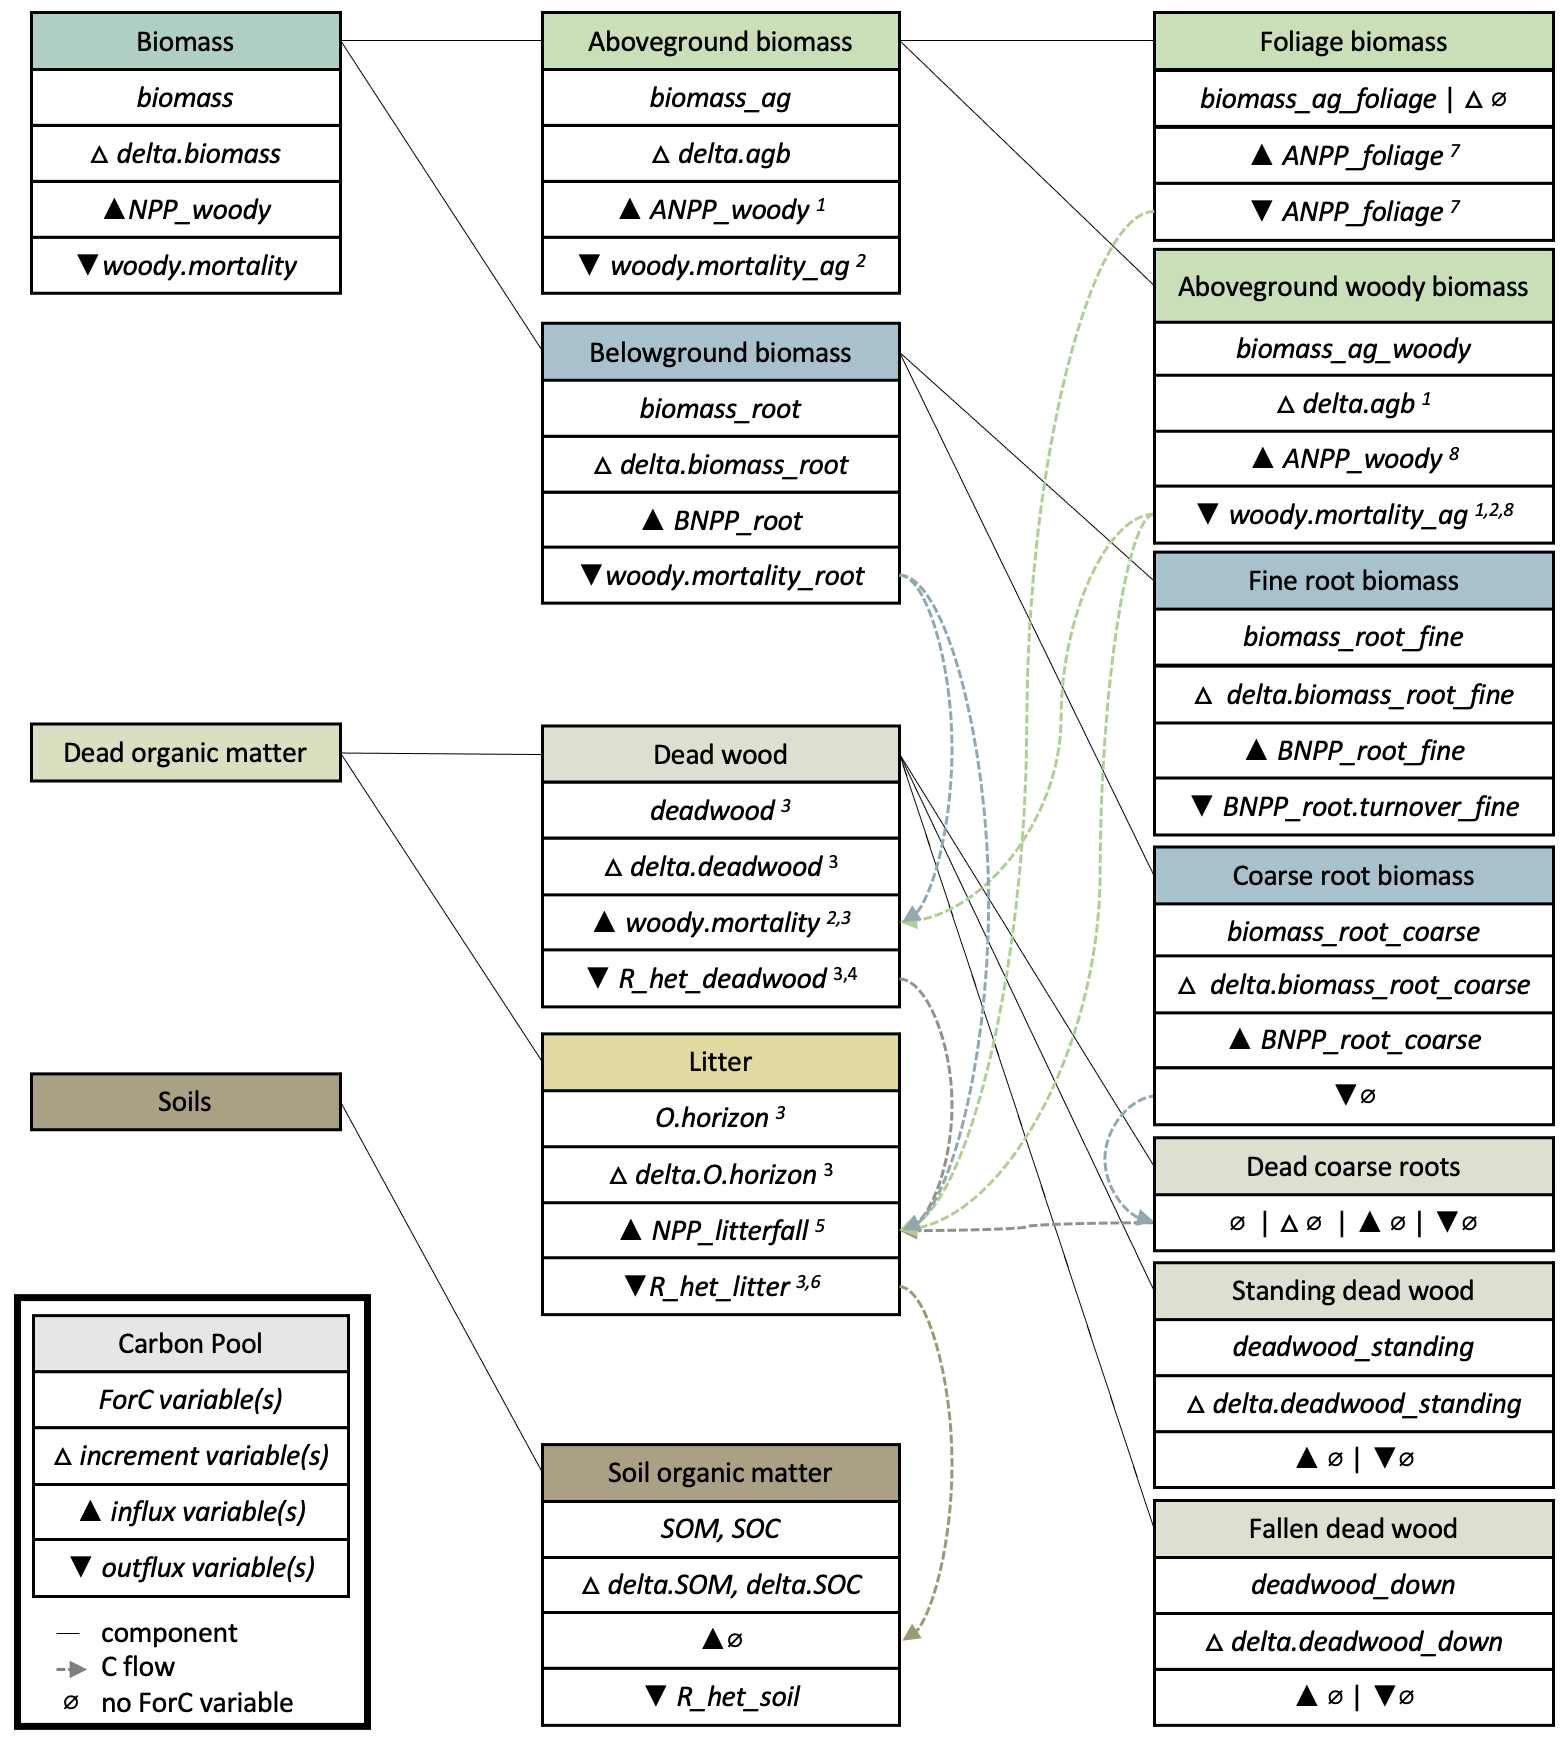
\includegraphics[width=14cm]{figures_tables/C_variable_mapping} \caption{\textbf{Schematic illustrating the carbon pools quantified under IPCC accounting; ForC variables corresponding to the stock, increment, influx and outflux; and relationships among them.} Correspondence of ForC variables to IPCC criteria often depends upon measurement protocols (e.g., min DBH). Additional caveats are as follows: (a,b) branch fall and mortality of stems below census min DBH, which are necessary for a full accounting of dead organic matter production but typically assumed negligible for calculations of biomass change, are excluded by common measurement practice (a) or ForC variable definition (b); (c) assumes that leaf production equals leaf fall, and that changes in foliage biomass are negligble; (d,e) belowground components excluded by common measurement practice (d) or ForC variable definition (e); (f) excludes movement of dead wood into litter through breakage or size reduction; (g) measurements often limited to litter horizon (OL) and may exclude larger branches and stems classified as litter and/or the more decomposed layers of the O horizon.}\label{fig:fig_variable_mapping}
\end{figure}

\subsubsection{Biomass}

Biomass includes living vegetation, above- and below-ground, both woody
and herbaceous, but with a focus on woody plants and trees given their
much greater potential to sequester large amounts of C
\citep{ipcc_2006_2006}.

Aboveground biomass, which is typically \textless200 t C
ha\textsuperscript{-1} but can exceed 700 t C ha\textsuperscript{-1}
\citep{anderson-teixeira_carbon_2021}, is defined by the IPCC as ``all
biomass of living vegetation above the soil including stems, stumps,
branches, bark, seeds, and foliage''
\citep{ipcc_good_2003, ipcc_2006_2006}. IPCC's guidance is that the
understory may be excluded the understory if it constitutes a ``minor''
component, \emph{where quantitative definitions of ``understory'' and
``minor'' are not provided}, but where a commonly applied minimum size
sampling threshold for mature forests would be 10 cm stem diameter at
breast height (DBH). A recent study characterizing the contributions of
trees in different DBH classes to ecosystem C stocks and fluxes found
that trees 1 - 10 cm DBH contributed up to \textasciitilde8\%
aboveground biomass, \textasciitilde17\% aboveground woody net primary
productivity (\(ANPP_{woody.stem}\)), and \textasciitilde20\% woody
mortality (\(M_{woody}\)) of mature closed-canopy forests worldwide
\citep{piponiot_distribution_2022}. In regrowth forests, woodlands, or
savannas, small trees and shrubs contribute a much larger proportion of
C stocks and fluxes \citep{piponiot_distribution_2022, refs}, and,
correspondingly, biomass estimates for these ecosystems tend include
smaller size classes \citep[e.g.,][]{refs}. Beyond the minimum DBH
sampled, forest censuses and biomass estimates also differ in their
inclusion of life forms other than dicot trees -- including lianas,
ferns, palms, and bamboo -- which in some places can reach large sizes
and/or constitute a large fraction of forest C. \emph{{[}explain IPCC
guidance{]}} Further, it is important to note that this excludes
standing dead wood, which is included in remote sensing biomass
estimates \citep{duncanson_aboveground_2021}.

A universal challenge in estimating biomass (living or dead) from forest
census data is applying appropriate allometries to convert DBH
measurements to biomass. Selection of allometries has an enormous
influence on estimates of biomass stocks, increments, of fluxes
\citep{clark_landscapescale_2000, clark_net_2001}. While trusted and
standardized allometric equations are becoming increasingly available
\citep{chave_improved_2014, rejou-mechain_biomass_2017, gonzalez-akre_allodb_2022},
large uncertainties remain. \emph{{[}explain IPCC guidance{]}}

Belowground biomass is defined as ``all biomass of live roots''
\citep{ipcc_good_2003, ipcc_2006_2006}, a definition including both
coarse roots, whose biomass is typically estimated based on stem
censuses and allometries or belowground to aboveground biomass ratios,
and fine roots, whose biomass is typically estimated via extraction of
roots from soil samples. The former, which is typically \textless40 t C
ha\textsuperscript{-1} \citep{anderson-teixeira_carbon_2021}, is
methodologically linked to aboveground biomass estimates, sharing the
same methodological sources of variation, but tending to be far more
uncertain. Fine root biomass generally constitutes a much smaller C pool
\citep[typically \textless5 t C
ha\textsuperscript{-1},][]{anderson-teixeira_carbon_2021}, and IPCC
guidance is that it can be excluded when fine roots cannot be
distinguished empirically from soil organic matter or litter
\citep{ipcc_2006_2006}, which can be a painstaking process. Field
methods for estimating root biomass are highly variable. IPCC's default
method for Tier 1 estimates is to apply a ratio of belowground to
aboveground biomass, with default factors defined based on ecological
zone, continent, and forest age \citep{ipcc_2006_2006, ipcc_2019_2019}.

\subsubsection{Dead Organic Matter}

Dead organic matter includes all non-living biomass that is not within
the mineral soil layer and smaller than the litter size threshold. It's
inclusion in inventories is not required under Tier 1 methodology for
Forest Land remaining Forest Land (see section 2.2), but is required for
land that has transitioned to or from forest within the past 20 years
\citep{ipcc_2006_2006}.

Dead wood, which is typically \textless50 t C ha\textsuperscript{-1} but
can exceed 150 t C ha\textsuperscript{-1}
\citep{anderson-teixeira_carbon_2021}, is defined by IPCC as ``all
non-living woody biomass not contained in the litter, either standing,
lying on the ground, or in the soil''
\citep{ipcc_good_2003, ipcc_2006_2006}. This pool includes standing and
fallen dead wood, stumps, and dead roots of diameter ≥10 cm (or a
diameter specified by the country). While dead wood stocks and fluxes
can be quite variable across forests
\citep{anderson-teixeira_carbon_2021}, and can at times be the dominant
pool in a forest ecosystem {[}e.g., following a severe natural
disturbance; \citet{carmona_coarse_2002}{]}, aboveground dead wood
remains relatively poorly characterized at a global scale
\citep{anderson-teixeira_carbon_2021}, and belowground dead wood is
rarely studied \citep{merganicova_dadwood_2012}. In turn, they are
poorly characterized in large-scale forest C budgets
\citep{pan_large_2011, harris_global_2021}, and IPCC's latest Tier 1
default values are based on just 1-31 references per climate zone
\citep[Table 2.2 in][]{ipcc_2019_2019}.

Litter, which is typically \textless40 t C ha\textsuperscript{-1} but
can exceed 100 t C ha\textsuperscript{-1}
\citep{anderson-teixeira_carbon_2021}, is defined by IPCCC as including
``all non-living biomass with a diameter less than a minimum diameter
chosen by the country (for example 10 cm), lying dead, in various states
of decomposition above the mineral or organic soil''
\citep{ipcc_good_2003, ipcc_2006_2006}. As noted above, live fine roots
may be included in litter when difficult to separate empirically. The
definition includes the entire O horizion, including litter (OL), fumic
(OF), and humic (OH) layers, in addition to litter embedded within the
soil. This definition contrasts with empirical studies that focus on
aboveground litter, often including only the OL layer in the definition
of litter, and do not always specify the components included. Similar to
dead wood, litter is poorly characterized in large-scale forest C
budgets \citep{pan_large_2011, harris_global_2021}, and IPCC's latest
Tier 1 default values are based on just 1-7 references per climate zone
\citep[Table 2.2 in][]{ipcc_2019_2019}.

\subsubsection{Soil Organic Matter/ Carbon}

Soil organic matter/ carbon (SOM/ SOC), which \emph{(statistic on how
much C is typial)} \citep{ref}, is defined by IPCC as ``organic carbon
in mineral and organic soils (including peat) to a specified depth
chosen by the country and applied consistently through the time series''
\citep{ipcc_good_2003, ipcc_2006_2006}. Live fine roots (suggested
diameter cutoff of 2 mm) may be included with soil organic matter when
it is not feasible to distinguish them empirically. The greatest source
of methodological variation in measuring SOM/ SOC is sampling depth,
which has a suggested default of 30 cm but may vary by country provided
that consistent criteria are applied.

\subsection{Land use categories}

IPCC defines land-use categories to include six categories -- Forest
Land, Grassland, Wetlands, Cropland, Settlements, and Other Land
\citep{ipcc_2006_2006}. Sub-divisions include land that has remained in
a particular category for \textgreater20 years (e.g., Forest Land
remaining Forest Land) and land that has been converted from one
category to another in the past 20 years (e.g., Cropland converted to
Forest Land). Forest Land is defined as at least 10-30\% crown cover of
trees with potential to reach a minimum height of 2-5 m \emph{in situ}
\citep{ipcc_good_2003}. Definitions of forest are allowed to vary by
country, but must be applied consistently. Forest Land includes land
where vegetation temporarily falls below the threshold values for forest
(e.g., due to disturbance), but is expected to exceed those thresholds
in the future \citep{ipcc_good_2003}.

Inventories are conducted only for managed land, which is defined by
IPCC to include ``all forests subject to some kind of human interactions
(notably commercial management, harvest of industrial round-wood (logs)
and fuelwood, production and use of wood commodities, and forest managed
for amenity value or environmental protection if specified by the
country), with defined geographical boundaries'' \citep{ipcc_good_2003}.
As such, managed land constitutes all or the majority of Forest Land in
most countries; however, many countries have not yet reported their
approach for defining managed land
\citep{ogle_delineating_2018, deng_comparing_2021}.

\section{Mapping ForC to EFDB}

ForC data is incredibly valuable to EFDB and there is data which is
included in the ForC database that does not meet EFDB standards. There
were two main EFDB guidelines which limits the amount of data we could
transfer. EFDB will not accept data which has been digitized(from graph)
and ForC does.

\subsection{Carbon cycle variables}

Mapping of variables is shown in Fig. 1.

\subsection{Land use categories}

Documented at
https://github.com/forc-db/IPCC-EFDB-integration/blob/main/doc/ForC-EFDB\_mapping/defining\_land\_subcategory.md,
https://github.com/forc-db/IPCC-EFDB-integration/blob/main/doc/ForC-EFDB\_mapping/IPCC\_LandUse\_mapping.csv,
and in
\href{https://github.com/forc-db/IPCC_database_integration/issues/8}{issue
\#8}.

The UNFCCC requires greenhouse gas reporting for all managed lands in a
country, where management is defined as ``human interventions and
practices have been applied to perform production, ecological or social
functions'' {[}\emph{IPCC 2006 full report REF}{]}. This definition is
applied differently across countries, and is not clearly defined by the
majority of governments \citep{ogle_delineating_2018}. Given this, and
because the IPCC definition of management does not necessarily match
that which would be reported in scientific publications and hence in
ForC, we do not transfer any classification of land management status
from ForC to the EFDB, but do provide auxiliary info that may be useful
in making this determination (e.g., geographical location).

\section{Updates to ForC (ForC v4.0)}

To support export of data to EFDB, and to improve the overall quality of
the ForC database, we defined \#\# new variables, implemented some
modest restructuring, resolved duplicate records, and conducted quality
control. This section describes changes relative to ForC v2.0
\citep{anderson-teixeira_forc_2018}.

\subsection{Defining new variables}

We added eleven increment variables to the set of named and defined
variables (or 22, counting \_OM and \_C versions), which previously
included only one (aboveground biomass increment, \emph{delta.agb}).
\emph{(https://github.com/forc-db/IPCC-EFDB-integration/issues/6)} These
are directly related to C stocks as previously defined in ForC, with
``\emph{delta.}'' added in front of the variable name.

Although these variables currently lack records, the structure exists
such that records can be populated over time.

To provide better definition of the previously existing variable
\emph{organic.layer}, which has a nebulous definition that reflects the
varied definitions adopted by original studies, we added two clearly
defined variables: \emph{litter} (relatively undecomposed plant
material/ OL horizon), and \emph{O.horizon} (entire O-horizon, including
\emph{litter} (OL)).

\subsection{Quality control measures}

Prior to releasing ForC v4.0, we executed several quality control
measures. First, we implemented a system of continuous integration using
GitHub Actions (\emph{sensu} Kim et al.~in review) to run some automatic
checks any time the master data files are updated. Second, to improve
information on geographic coordinates, we flagged and reviewed records
with suspected low precision \emph{(Issue
\#29){[}https://github.com/forc-db/ForC/issues/229{]}}. Third, to
identify erroneous climate data\ldots{} \emph{(Issue
\#212){[}https://github.com/forc-db/ForC/issues/212{]}}.

\subsection{Resolving duplicates}

Because ForC v4.0 contained known duplicate records, we used R scripts
to remove likely duplicates, as detailed in
\citet{anderson-teixeira_carbon_2021}. Henceforth, we refer to the
records with duplicates removed as ``independent records''.

\subsection{Manual review of records to be sent to EFDB}

EFDB data submissions require information that was not recorded in
previous versions of ForC. It was therefore necessary to return to
original publications to retrieve relevant information, including
\ldots{}

\section{Results}

\subsection{ForC v4.0 contents}

As of April 15, 2022, ForC (v4.0) contained NA independent records (NA
total), NA of which were for variables relevant to EFDB (Fig. 1). These
records were distributed across all forested continents and ecozones,
with particularly high concentrations in \emph{{[}ecozone(s){]}} and low
concentrations in \emph{{[}ecozone(s){]}} (Fig. 2). The most widely
represented forest type was \emph{{[}type{]}}, followed by
\emph{{[}type{]}} and \emph{{[}type{]}} (Fig. 3).

\begin{figure}
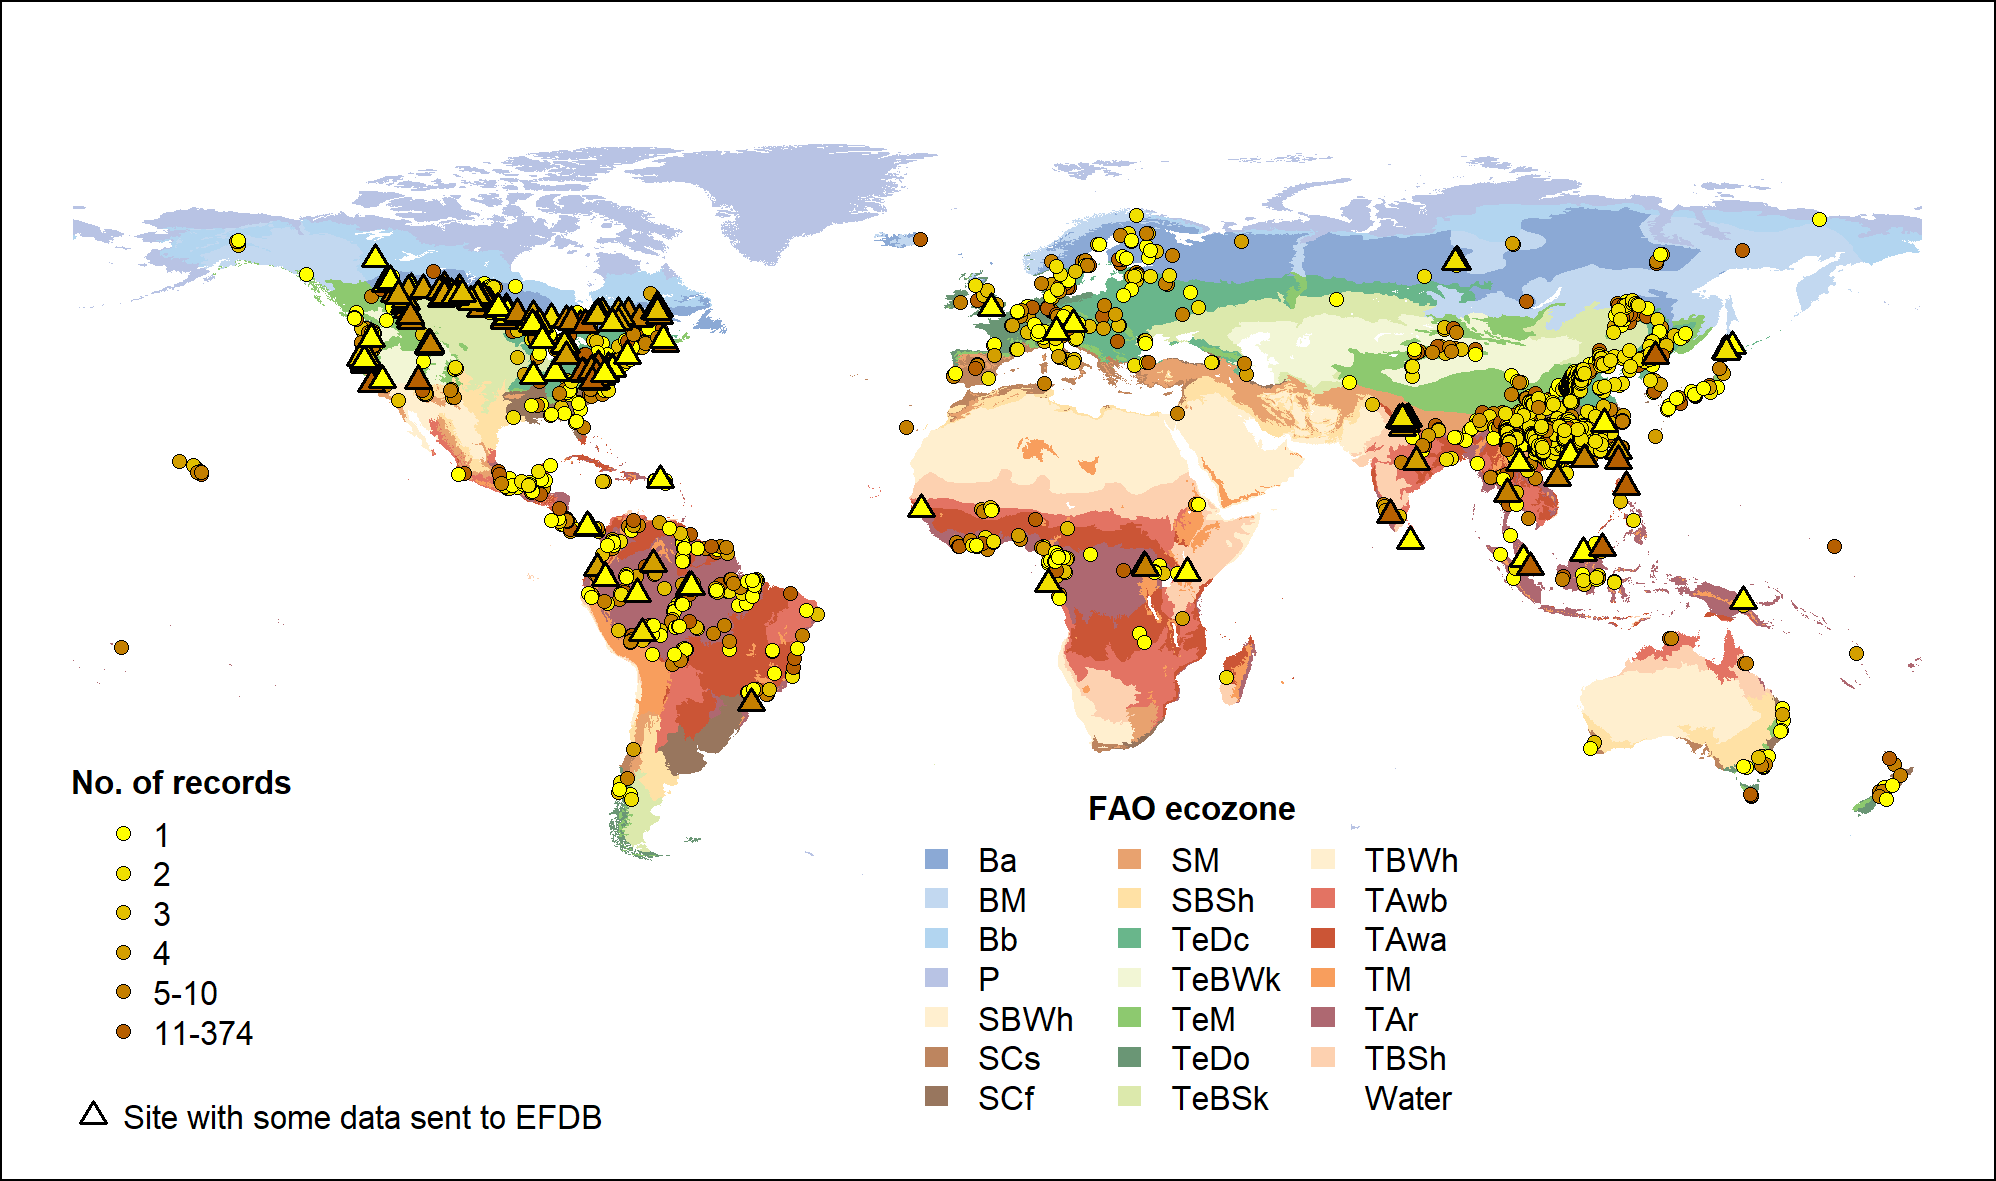
\includegraphics[width=15cm]{figures_tables/World_Map_of_sites_with_FAO_and_IPCC_data_sent} \caption{\textbf{Map of sites in ForC shaded by number of records relevant to (circles) and transferred to (triangles) EFDB.} Symbols are colored according to the number of records at each site. Underlying map shows FAO ecozones, which are coded as follows: ....}\label{fig:fig_map}
\end{figure}

\begin{figure}
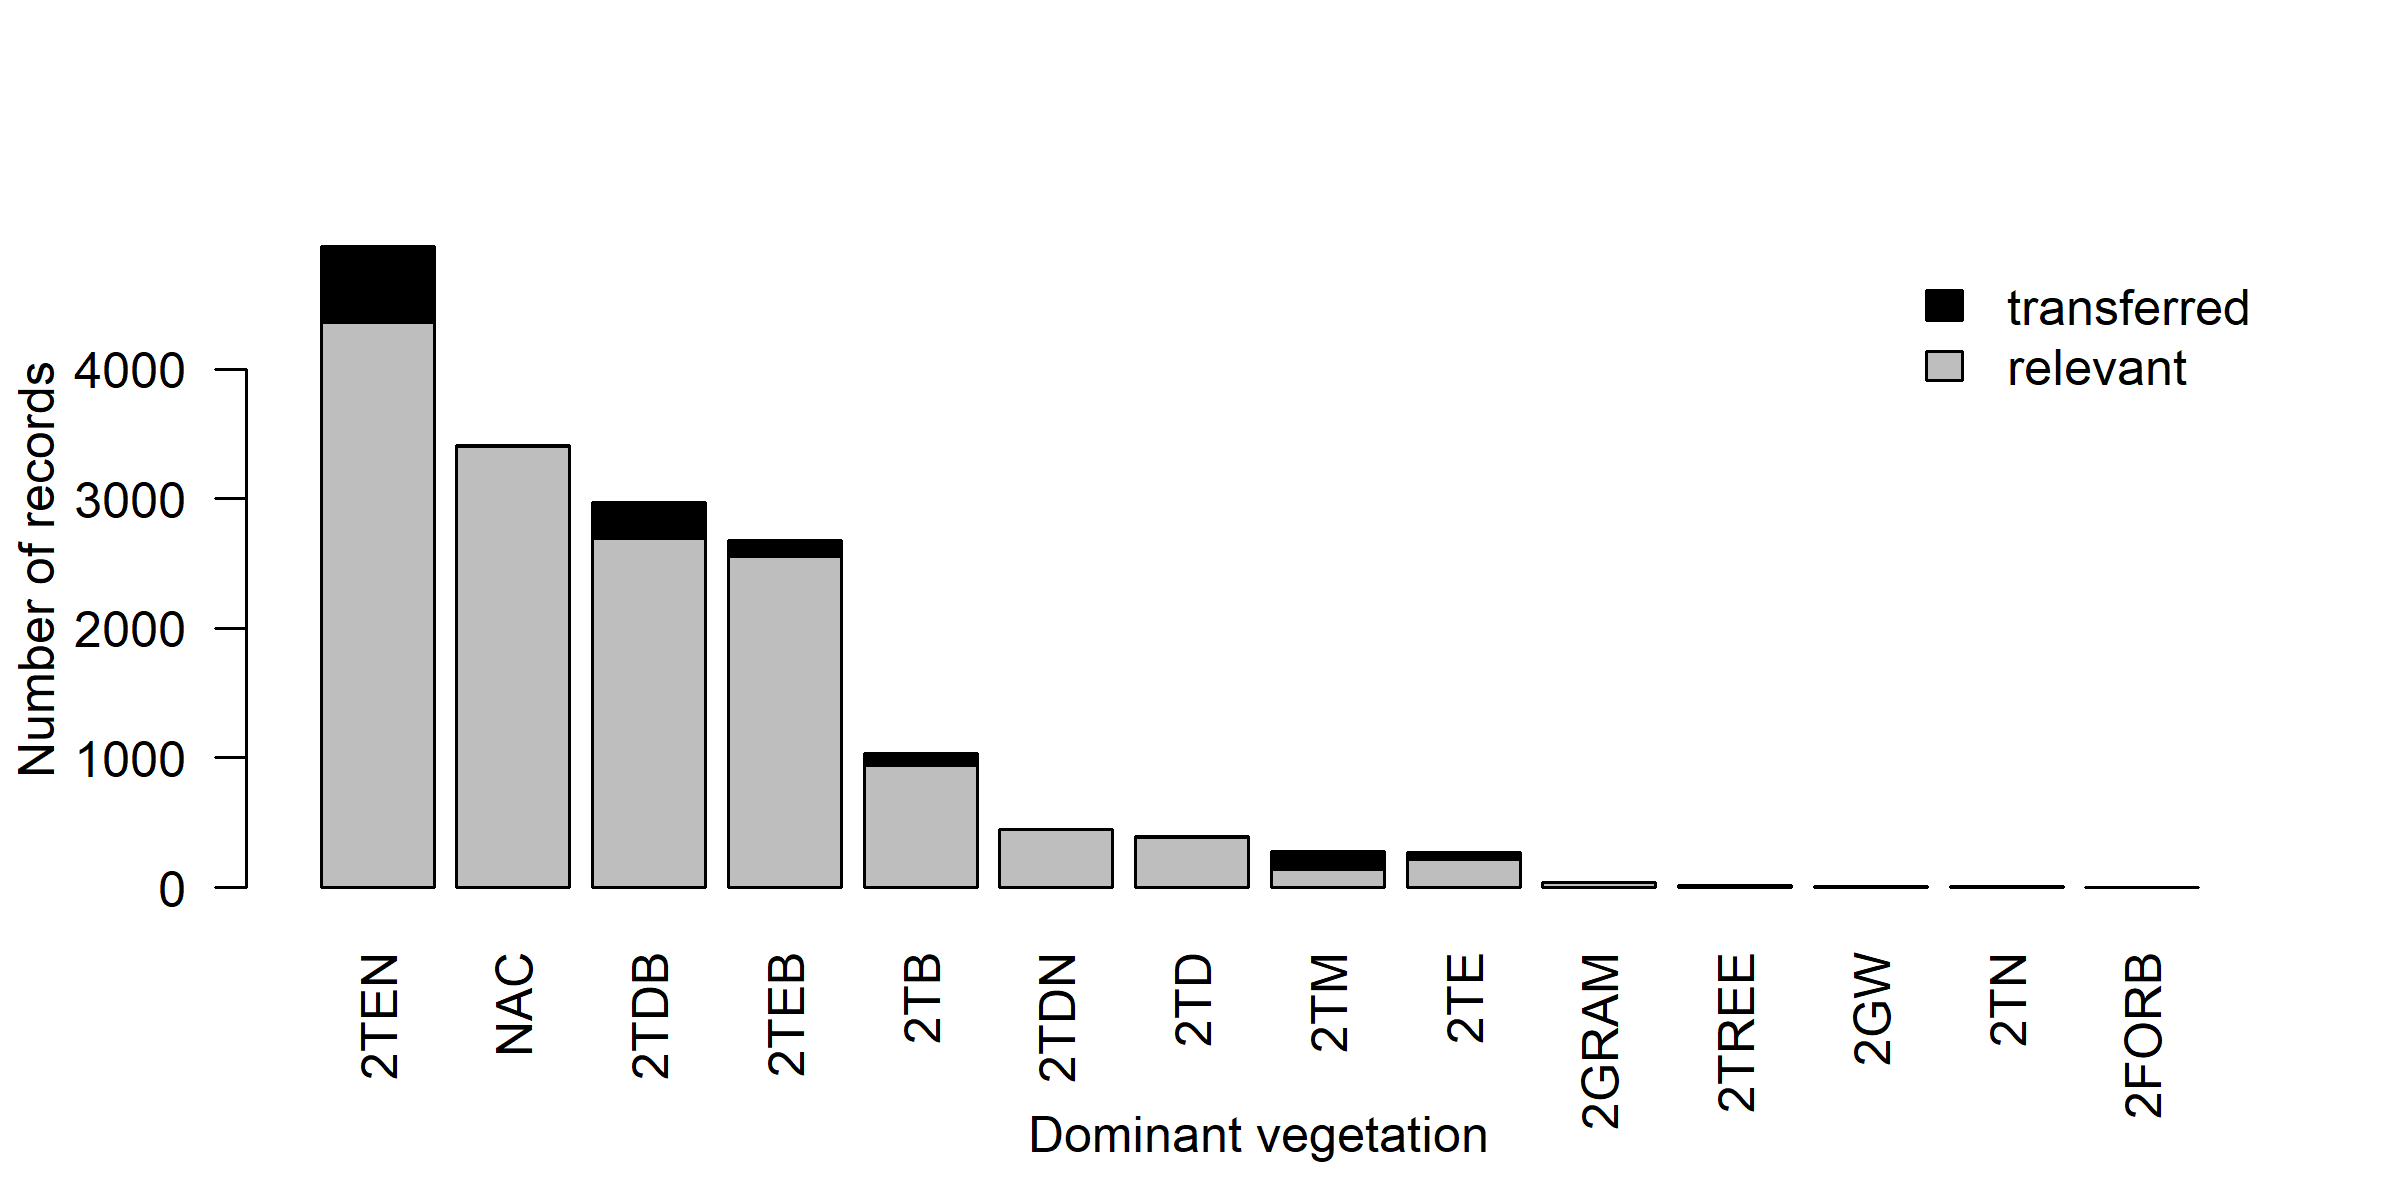
\includegraphics[width=15cm]{figures_tables/Histogram_n_Relevant_and_Transferred_Records} \caption{\textbf{Histograms of number of records in ForC relevant to (grey) and transferred to (black) EFDB, organized by (a) dominant vegetation type, (b) FAO ecozone, (c) continent, and (d) stand age.} For dominant vegetation (a), 'Other' includes deciduous needleleaf, mixed broadleaf- needleleaf, non-woody vegetation (e.g., early successional), and incompletely classified or mixed forest types. For FAO ecozones (b), codes are as listed in the caption of Figure 2.}\label{fig:fig_dominant_veg}
\end{figure}

ForC contained data for \textbf{\#\#} of the \textbf{\#\#} variables
relevant to EFDB (Table 2, Fig. 1).

\begin{longtabu} to \linewidth {>{\raggedright}X>{\raggedright}X>{\raggedright}X>{\raggedright}X>{\raggedright}X}
\caption{\label{tab:table_variables}\textbf{Numbers of records of ForC variables relevant to, and sent to, EFDB.} Relationships of variables to IPCC-defined forest C pools (Table 1) and to each other are illustrated in Figure 1. }\\
\hline
\textbf{variable} & \textbf{n in ForC} & \textbf{n independent records in ForC} & \textbf{n reviewed} & \textbf{n sent to EFDB}\\
\hline
\textbf{Biomass} & \textbf{} & \textbf{} & \textbf{} & \textbf{}\\
\hline
biomass &  &  &  & \\
\hline
delta.biomass &  &  &  & \\
\hline
NPP\_woody &  &  &  & \\
\hline
woody.mortality &  &  &  & \\
\hline
\textbf{Aboveground biomass} & \textbf{} & \textbf{} & \textbf{} & \textbf{}\\
\hline
biomass\_ag &  &  &  & \\
\hline
biomass\_ag\_woody &  &  &  & \\
\hline
biomass\_ag\_foliage &  &  &  & \\
\hline
delta.agb &  &  &  & \\
\hline
ANPP\_woody &  &  &  & \\
\hline
ANPP\_foliage &  &  &  & \\
\hline
woody.mortality\_ag &  &  &  & \\
\hline
\textbf{Belowground biomass} & \textbf{} & \textbf{} & \textbf{} & \textbf{}\\
\hline
biomass\_root &  &  &  & \\
\hline
biomass\_root\_fine &  &  &  & \\
\hline
biomass\_root\_coarse &  &  &  & \\
\hline
delta.biomass\_root &  &  &  & \\
\hline
delta.biomass\_root\_coarse &  &  &  & \\
\hline
delta.biomass\_root\_fine &  &  &  & \\
\hline
woody.mortality\_root &  &  &  & \\
\hline
BNPP\_root\_fine &  &  &  & \\
\hline
BNPP\_root.turnover\_fine &  &  &  & \\
\hline
BNPP\_root\_coarse &  &  &  & \\
\hline
\textbf{Dead wood} & \textbf{} & \textbf{} & \textbf{} & \textbf{}\\
\hline
deadwood &  &  &  & \\
\hline
deadwood\_standing &  &  &  & \\
\hline
deadwood\_down &  &  &  & \\
\hline
delta.deadwood &  &  &  & \\
\hline
delta.deadwood\_standing &  &  &  & \\
\hline
delta.deadwood\_down &  &  &  & \\
\hline
R\_het\_deadwood & 0 &  &  & \\
\hline
\textbf{Litter} & \textbf{} & \textbf{} & \textbf{} & \textbf{}\\
\hline
O.horizon &  &  &  & \\
\hline
delta.O.horizon &  &  &  & \\
\hline
litter &  &  &  & \\
\hline
delta.litter &  &  &  & \\
\hline
NPP\_litterfall &  &  &  & \\
\hline
R\_het\_litter &  &  &  & \\
\hline
\textbf{Soil organic matter} & \textbf{} & \textbf{} & \textbf{} & \textbf{}\\
\hline
SOM / SOC &  &  &  & \\
\hline
delta.SOM / delta.SOC &  &  &  & \\
\hline
R\_het\_soil &  &  &  & \\
\hline
\textbf{TOTAL} & \textbf{} & \textbf{} & \textbf{} & \textbf{}\\
\hline
\end{longtabu}

\subsection{Data transfers to EFDB}

As of April 15, 2022, we had reviewed and sent NA, NA of which have been
reviewed, accepted, and posted (Fig. 2-3, Table 2). \emph{{[}DETAILS{]}}

\section{Recommendations}

(\emph{strongly flag both useful variables that the EFDB does not track
and useful variables that papers fail to include that EFDB needs})

\subsection{Data collection and analysis needs}

\emph{(Paragraph highlighting important gaps in variables / regions)}

Several variables of value to IPCC, including standing dead wood, woody
mortality, delta.agb, are not calculated and presented as frequently as
are AGB and ANPP\_woody, even though they can readily be derived from
the same census data. We recommend that researchers calculate and report
these, following the reporting guidelines specified below. Furthermore,
there is an opportunity to fill data gaps by calculating these from
existing census data. For example, the core census protocol of the
Forest Global Earth Observatory {[}ForestGEO;
\citet{anderson-teixeira_ctfsforestgeo_2015},\citet{davies_forestgeo_2021}{]}
collects the data required to calculate standing dead wood, woody
mortality, and delta.agb, but these have not been calculated and
reported for all sites for which the appropriate number of censuses are
available \citep[but see][\citet{refs}]{piponiot_distribution_2022}.

Given widespread trends of increasing tree mortality\citep{refs},
including through severe natural disturbance \citep{refs}, better
characterization of dead wood will be critical.

\subsection{Data reporting needs}

We recommend that, unless they have some specific reason to do
otherwise, researchers calculate and report the values according to IPCC
standards:

\begin{itemize}
\item
  adopt common standards for variables like min diameter of deadwood,
  select soil sampling increments to include a cutoff at 30.
\item
  report 95\% CIs, SE, or STD and n
\item
  report C variables in article text, table, or SI table. EFDB cannot
  accept data digitized from figures
\item
  present calculations of all variables that would be useful to IPCC.
  EFDB requires that data in the database be presented in the original
  article, and as such cannot accept subsequent calculations. For
  example, if aboveground biomass and total biomass are presented, but
  root biomass is not presented, root biomass cannot be subsequently
  calculated and sent to EFDB. Similarly, fine and coarse root biomass
  can't be summed; soil carbon can't be summed across depth increments,
  etc.
\end{itemize}

For data synthesis projects, compilation can only be useful to the EFDB
if they include all the required, along with transparent description on
the methodology applied to derive emission factors (or have a brief
description and a reference to the original source) and the original
emission factor values are present (not modified/rounded).

\textbf{Contributing data to ForC and/or EFDB directly will ensure its
broader impact.} The latter is more efficient for getting data to EFDB,
but does not get the data into ForC, where it can be more broadly
useful--for example, being used for basic science
\citep[e.g.,][]{banburymorgan_global_2021, anderson-teixeira_carbon_2021}
or model benchmarking \citep{fer_ecosystem_2021}.

\subsection{Database needs}

There are plenty of relevant, published data that are not included in
ForC. Systematic review of the literature could vastly improve data
coverage. \emph{(There are some efforts underway, including a few that
Susan can specify.)}

\subsection{IPCC protocol considerations}

An important challenge is that forests are changing rapidly, and data
collected a decade ago may no longer be relevant, particularly in the
cases of C increments and fluxes.

Remote sensing biomass estimates include standing dead wood
\citep{duncanson_aboveground_2021}.

\section{Conclusions}

\clearpage

\section{Appendix A}

\begin{longtabu} to \linewidth {>{\raggedright}X>{\raggedright}X>{\raggedright}X>{\raggedright}X>{\raggedright}X}
\caption{\label{tab:table_ForCfieldmapping}\textbf{Mapping of ForC fields to EFDB.} See footnotes at end of table (still need to be properly inserted). }\\
\hline
\textbf{ForC table} & \textbf{ForC field} & \textbf{EFDB field} & \textbf{Usage} & \textbf{Required}\\
\hline
\endfirsthead
\caption[]{\textbf{Mapping of ForC fields to EFDB.} See footnotes at end of table (still need to be properly inserted).  \textit{(continued)}}\\
\hline
\textbf{ForC table} & \textbf{ForC field} & \textbf{EFDB field} & \textbf{Usage} & \textbf{Required}\\
\hline
\endhead
Measurements & measurement.ID & Other Properties & direct mapping & (no)\\
\hline
 & dominant.life.form & 1996 Source/Sink Categories, 2006 Source/Sink Categories & used to determine land subcategories (see defining\_land\_subcategory.md) & yes\\
\hline
 & stand.age & 1996 Source/Sink Categories, 2006 Source/Sink Categories, Parameters/ Conditions & used to determine land subcategories (see defining\_land\_subcategory.md), directly listed in Parameters/ Conditions & (yes)\\
\hline
 & dominant.veg, veg.notes, min.dbh & Parameters/ Conditions & direct mapping/ linking to dominant.veg description & no\\
\hline
 & variable.name & - & link to variable info in ForC\_variables table & yes\\
\hline
 & date / start.date, end.date & Other Properties & direct mapping & no\\
\hline
 & mean & Value & direct mapping & yes\\
\hline
 & mean.in.original.units & Value in Common Units & direct mapping & yes\\
\hline
 & original.units & Common Unit & direct mapping & yes\\
\hline
 & lower95\%CI, upper 95\%CI, se, sd and n & Lower Confidence Limit, Upper Confidence Limit & direct or calculated & (yes)\\
\hline
 & depth, covariate\_1, cov\_1.value, covariate\_2, cov\_2.value & Other Properties & direct mapping & no\\
\hline
 & allometry\_1, allometry\_2 & Comments from Data Provider & link to biomass allometry source, when provided & no\\
\hline
 & data.location.within.source & - & confirm that data weren't digitized, facilitate finding data in original publication & yes\\
\hline
 & ForC.investigator & Data Provider, Data Provider Contact & link to Data Provider, Data Provider Contact info & yes\\
\hline
Sites & site.ID, sites.sitename & Other Properties & direct mapping & (no)\\
\hline
 & lat, lon & Region/Regional conditions & direct mapping; used to extract continent, Koeppen, and FAO.ecozone & (no)\\
\hline
 & country, state, city, masl,  mat, map & Region/Regional conditions & direct mapping & no\\
\hline
 & continent, Koeppen & Region/Regional conditions & direct mapping & auto\\
\hline
 & soil.texture, sand, silt, clay, soil.classification & Parameters/ Conditions & direct mapping & no\\
\hline
 & FAO.ecozone & Parameters/ Conditions & direct mapping & auto\\
\hline
History & date, hist.cat, hist.type & 1996 Source/Sink Categories, 2006 Source/Sink Categories, Abatement/Control technologies & used to determine distmrs.type for Source/Sink Categories, generate list of events for Abatement/Control technologies & (yes)/no**\\
\hline
 & plot.area & Other Properties & direct mapping & no\\
\hline
Plots & plot.ID, plot.name & Other Properties & direct mapping & (no)\\
\hline
 & distmrs.type & 1996 Source/Sink Categories, 2006 Source/Sink Categories & used to determine land subcategories (see defining\_land\_subcategory.md) & auto\\
\hline
 & distmrs.type, distmrs.year, regrowth.type, regrowth.year & Other Properties & direct mapping & auto\\
\hline
PFT & description & Parameters/ Conditions & direct mapping & auto\\
\hline
variables & variable.type & Gases & For stocks in unit of organic matter, gases include CO2, CO, CH4, NO, NO2, N2O. For increments, fluxes, and stocks in units of C, gases includes only CO2. & auto\\
\hline
 & variable.name & C pool, Equation & link to C pool, Equation & auto\\
\hline
 & description & Description & direct mapping & auto\\
\hline
 & extended.description & Other Properties & direct mapping & auto\\
\hline
 & units & Unit (ID) & link to IPCC units & auto\\
\hline
Citations & citation.citation & Full Technical Reference & direct mapping & yes/auto\\
\hline
 & citation.language & Reference Language & direct mapping & yes/auto\\
\hline
 & citation.url & URL & direct mapping & no/auto\\
\hline
 & citation.abstract & Abstract in English & direct mapping & no/auto\\
\hline
 & source.type & Source of Data & direct mapping & yes\\
\hline
\end{longtabu}

`Required' field indicates whether the field is required by EFDB: yes =
value required; (yes) = input required, missing value acceptable if not
reported; auto = present within ForC infrasructure, and therefore will
always be exported to EFDB ; (no) = not required for EFDB, but required
for ForC and therefore will always be exported to EFDB; no = not
required, but exported to EFDB when a value is present.

** `(yes)' for most recent severe disturbance; `no' for other history
events

\clearpage

\section{Appendix B}

\begin{longtabu} to \linewidth {>{\raggedright}X>{\raggedright}X>{\raggedright}X>{\raggedright}X>{\raggedright}X}
\caption{\label{tab:table_ForCchanges}\textbf{Table of changes to ForC fields.}}\\
\hline
\textbf{Table} & \textbf{Column} & \textbf{Description} & \textbf{Changes} & \textbf{Motivation}\\
\hline
\endfirsthead
\caption[]{\textbf{Table of changes to ForC fields.} \textit{(continued)}}\\
\hline
\textbf{Table} & \textbf{Column} & \textbf{Description} & \textbf{Changes} & \textbf{Motivation}\\
\hline
\endhead
Sites & coordinates.precision & Precision of geographic coordinates, as reported by source or estimated from maps. & field added & allow identification of records with poor coordinate precision\\
\hline
Measurements & data.location.within.source & Location of data within the source listed in citation.ID. & field added & facilitate review, ensure traceability\\
\hline
 & sd, se, lower95\%CI, upper 95\%CI & Standard deviation, standard error, and lower and upper 95 percent confidence intvervals, respectively. & replaces `stat` and `stat.name` & cleaner format; ability to handle assymetrical 95 percent confidence intervals\\
\hline
 & mean.in.original.units, original.units & mean value and units presented in original publication & fields added & provide IPCC with original units, reduce errors/improve reproducibility\\
\hline
 & C.conversion.factor & Assumed/ measured C content of organic matter used to convert organic matter to C. & field added & track units conversion, allow back-calculation of OM if conversion factor deemed inappropriate\\
\hline
PFT & description & Definition of the pftcode at the community level. Differs from individual level in that properly describes mixed plant functional types. & field added & \\
\hline
 & description.individual & Definition of the pftcode at the individual plant level. & field name change (previously `description`) & \\
\hline
Citations & citation.citation & Full citation. Most of these records are automatically generated in R based upon DOI lookup. & field added & field required by IPCC\\
\hline
 & citation.language & Language of original publication, automatically generated based on the title and abstract, with some manual entries and corrections. & field added & field required by IPCC\\
\hline
 & citation.url & URL of original publication, generally retrieved automatically via URL lookup. & field added & field required by IPCC\\
\hline
 & citation.abstract & Abstract, generally retrieved automatically via DOI lookup. & field added & field required by IPCC\\
\hline
 & source.type & citation source type & field added & field required by IPCC\\
\hline
 & pdf.in.repository & Indicates whether pdf of original study has been retrieved and saved in ForC's reference repository & field added & housekeeping\\
\hline
 & EFDB.ready & Indicates whether data have been checked for export to EFDB. & field added & housekeeping\\
\hline
\end{longtabu}



\codedataavailability{use this to add a statement when having data sets
and software code
available} %% use this section when having data sets and software code available



%%%%%%%%%%%%%%%%%%%%%%%%%%%%%%%%%%%%%%%%%%
%% optional

%%%%%%%%%%%%%%%%%%%%%%%%%%%%%%%%%%%%%%%%%%
\appendix
\section{Mapping ForC to EFDB}

CURRENT TABLE 3 GOES HERE

\section{Updates to ForC}

CURRENT TABLE 4 GOES HERE
\noappendix

%%%%%%%%%%%%%%%%%%%%%%%%%%%%%%%%%%%%%%%%%%
\authorcontribution{(fill this in)} %% optional section

%%%%%%%%%%%%%%%%%%%%%%%%%%%%%%%%%%%%%%%%%%
\competinginterests{The authors declare no competing
interests.} %% this section is mandatory even if you declare that no competing interests are present

%%%%%%%%%%%%%%%%%%%%%%%%%%%%%%%%%%%%%%%%%%

%%%%%%%%%%%%%%%%%%%%%%%%%%%%%%%%%%%%%%%%%%
\begin{acknowledgements}
Thank you to all researchers who collected and published the data
contained in ForC, and to all research assistants and collaborators who
have helped to build the database. Funding for this study was provided
by Bezos Earth Fund to The Nature Conservancy, the Institute for Global
Environmental Strategies, WLS(?)
\end{acknowledgements}

%% REFERENCES
%% DN: pre-configured to BibTeX for rticles

%% The reference list is compiled as follows:
%%
%% \begin{thebibliography}{}
%%
%% \bibitem[AUTHOR(YEAR)]{LABEL1}
%% REFERENCE 1
%%
%% \bibitem[AUTHOR(YEAR)]{LABEL2}
%% REFERENCE 2
%%
%% \end{thebibliography}

%% Since the Copernicus LaTeX package includes the BibTeX style file copernicus.bst,
%% authors experienced with BibTeX only have to include the following two lines:
%%
\bibliographystyle{copernicus}
\bibliography{references.bib}
%%
%% URLs and DOIs can be entered in your BibTeX file as:
%%
%% URL = {http://www.xyz.org/~jones/idx_g.htm}
%% DOI = {10.5194/xyz}


%% LITERATURE CITATIONS
%%
%% command                        & example result
%% \citet{jones90}|               & Jones et al. (1990)
%% \citep{jones90}|               & (Jones et al., 1990)
%% \citep{jones90,jones93}|       & (Jones et al., 1990, 1993)
%% \citep[p.~32]{jones90}|        & (Jones et al., 1990, p.~32)
%% \citep[e.g.,][]{jones90}|      & (e.g., Jones et al., 1990)
%% \citep[e.g.,][p.~32]{jones90}| & (e.g., Jones et al., 1990, p.~32)
%% \citeauthor{jones90}|          & Jones et al.
%% \citeyear{jones90}|            & 1990

\end{document}
